\documentclass[12pt,a4paper]{article}

% --- PACKAGES ---
\usepackage[utf8]{inputenc}
\usepackage[T1]{fontenc}
\usepackage[english]{babel}
\usepackage{geometry}
\usepackage{graphicx}
\usepackage{fancyhdr}
\usepackage{xcolor}
\usepackage{titlesec}
\usepackage{tcolorbox}
\usepackage{listings}
\usepackage{courier}
\usepackage{hyperref}
\usepackage{booktabs}
\usepackage{array}
\usepackage{caption}
\usepackage{float}
\usepackage{setspace}
\usepackage[dvipsnames]{xcolor}
\usepackage{tikz}
\usetikzlibrary{shapes,arrows,positioning,calc}

% --- PAGE SETUP ---
\geometry{top=2.5cm, bottom=2.5cm, left=2.8cm, right=2.8cm}
\setstretch{1.2}

% --- COLORS ---
\definecolor{primary}{HTML}{004AAD}
\definecolor{darkgray}{HTML}{333333}
\definecolor{codegreen}{HTML}{006400}
\definecolor{lightgray}{gray}{0.95}
\definecolor{codegray}{HTML}{f5f5f5}
\definecolor{stringpurple}{HTML}{A31515}
\definecolor{commentgray}{HTML}{6A737D}
\definecolor{dockerblue}{HTML}{2496ED}
\definecolor{nginxgreen}{HTML}{009639}

% --- HEADER AND FOOTER ---
\pagestyle{fancy}
\fancyhf{}
\fancyhead[L]{\textcolor{primary}{\textbf{Jala University}}}
\fancyhead[R]{\textcolor{primary}{\textbf{DevOps - 2025}}}
\fancyfoot[C]{\textcolor{darkgray}{\thepage}}
\renewcommand{\headrulewidth}{1pt}
\renewcommand{\headrule}{\color{primary}\hrule height 1pt \vspace{2pt}}

% --- SECTION TITLE FORMAT ---
\titleformat{\section}
 {\Large\bfseries\color{primary}}
 {}
 {0em}
 {}
 [\vspace{-0.3cm}\hrulefill\vspace{0.3cm}]
\titleformat{\subsection}
 {\large\bfseries\color{darkgray}}
 {}
 {0em}
 {}

% --- CODE STYLE ---
\lstdefinelanguage{Dockerfile}{
  keywords={FROM, RUN, CMD, LABEL, EXPOSE, ENV, ADD, COPY, ENTRYPOINT, VOLUME, USER, WORKDIR, ARG, ONBUILD, STOPSIGNAL, HEALTHCHECK, SHELL, AS, version, services, volumes, networks, build, context, dockerfile, image, container_name, ports, environment, depends_on, restart, healthcheck, test, interval, timeout, retries, driver, ipam, config, subnet, external, name},
  keywordstyle=\color{primary}\bfseries,
  sensitive=false,
  comment=[l]{\#},
  commentstyle=\color{commentgray}\itshape,
  stringstyle=\color{stringpurple},
  morestring=[b]",
  morestring=[b]'
}

\lstdefinestyle{custom}{
  backgroundcolor=\color{codegray},
  commentstyle=\color{commentgray}\itshape,
  keywordstyle=\color{primary}\bfseries,
  numberstyle=\tiny\color{gray},
  stringstyle=\color{stringpurple},
  basicstyle=\ttfamily\small\color{darkgray},
  breaklines=true,
  captionpos=b,
  numbers=left,
  numbersep=8pt,
  frame=single,
  framerule=0.6pt,
  rulecolor=\color{lightgray},
  xleftmargin=10pt,
  xrightmargin=10pt,
  showstringspaces=false,
  tabsize=2
}

\lstdefinestyle{bash}{
  style=custom,
  language=bash,
  keywordstyle=\color{dockerblue}\bfseries,
  morekeywords={docker, curl, openssl, ls, cat, echo, sleep, ps, exec, ping}
}

% --- DOCUMENT ---
\begin{document}

\begin{center}
 {\Huge \textbf{Laboratory Week 3 - Docker Compose}}\\[0.4cm]
 \rule{\textwidth}{0.8pt}\\[0.4cm]
\end{center}

% --- COURSE INFORMATION ---
\section*{Course Information}
\begin{tabular}{@{}>{\bfseries}l@{\hspace{0.5cm}}l@{}}
\toprule
University & Jala University \\
Course & [Official - ES] - Development and Operations - CSDV-246 \\
Section & B \\
Professor & Richard Lopez \\
Faculty Practitioner & Miguel Montalvo \\
\bottomrule
\end{tabular}

\vspace{0.5cm}

% --- STUDENT INFORMATION ---
\section*{Student Information}
\begin{tabular}{@{}>{\bfseries}l@{\hspace{0.5cm}}l@{}}
\toprule
Student & Shadith Cuenca Kuno \\
Date & November 2025 \\
\bottomrule
\end{tabular}

\vspace{0.5cm}

\section{Objective}

Learn to manage multi-container applications declaratively using Docker Compose, allowing versioning of configurations and simplifying environment replicability through Docker networks.

\section{Architecture Overview}

\begin{center}
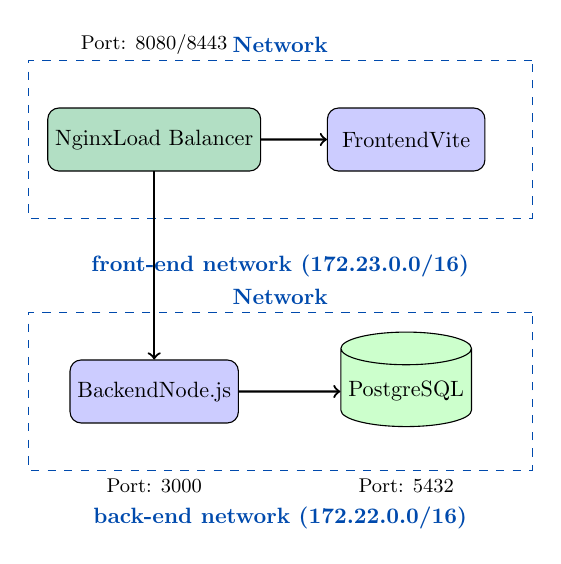
\begin{tikzpicture}[scale=0.8, transform shape]
    % Define styles
    \tikzstyle{service} = [rectangle, rounded corners, minimum width=2.5cm, minimum height=1cm, text centered, draw=black, fill=blue!20]
    \tikzstyle{database} = [cylinder, shape border rotate=90, draw=black, minimum height=1.5cm, minimum width=2cm, fill=green!20, aspect=0.25]
    \tikzstyle{network} = [rectangle, dashed, draw=primary, minimum width=8cm, minimum height=2.5cm, label=above:\textcolor{primary}{\textbf{Network}}
    ]

    % Front-end network
    \node[network] (frontend-net) at (0,3) {};
    \node[service, fill=nginxgreen!30] (lb) at (-2,3) {Nginx\\Load Balancer};
    \node[service] (frontend) at (2,3) {Frontend\\Vite};
    \node[above of=lb, node distance=1.5cm] {\small Port: 8080/8443};

    % Back-end network
    \node[network] (backend-net) at (0,-1) {};
    \node[service] (backend) at (-2,-1) {Backend\\Node.js};
    \node[database] (db) at (2,-1) {PostgreSQL};
    \node[below of=backend, node distance=1.5cm] {\small Port: 3000};
    \node[below of=db, node distance=1.5cm] {\small Port: 5432};

    % Connections
    \draw[->, thick] (lb) -- (frontend);
    \draw[->, thick] (lb) -- (backend);
    \draw[->, thick] (backend) -- (db);

    % Network labels
    \node[below of=frontend-net, node distance=2cm] {\textcolor{primary}{\textbf{front-end network (172.23.0.0/16)}}};
    \node[below of=backend-net, node distance=2cm] {\textcolor{primary}{\textbf{back-end network (172.22.0.0/16)}}};
\end{tikzpicture}
\end{center}

\newpage

\section{Step 1: Create compose.yml for Backend with Database}

A Docker Compose file was created to orchestrate the backend application and PostgreSQL database with proper networking and persistence.

\begin{tcolorbox}[colback=lightgray, colframe=dockerblue, title=\textbf{compose.yml - Backend Configuration}, fonttitle=\bfseries, coltitle=white, center title]
\begin{lstlisting}[style=bash, caption={Validating compose configuration}]
docker-compose -f compose.yml config
\end{lstlisting}
\begin{center}
    \includegraphics[width=0.9\textwidth]{compose-config.png}
\end{center}
\end{tcolorbox}

\subsection{Configuration Features}
\begin{itemize}
    \item \textbf{Multi-service orchestration}: Backend Node.js + PostgreSQL
    \item \textbf{Health checks}: Automatic monitoring of service availability
    \item \textbf{Environment variables}: Secure configuration management
    \item \textbf{Service dependencies}: Controlled startup order
\end{itemize}

\section{Step 2: Configure Data Persistence and Network}

\subsection{Volume Configuration}
A persistent volume was configured for the PostgreSQL database to ensure data persistence across container restarts.

\begin{tcolorbox}[colback=lightgray, colframe=primary, title=\textbf{Volume and Network Setup}, fonttitle=\bfseries, coltitle=white, center title]
\begin{lstlisting}[style=bash, caption={Docker volumes and networks}]
# List volumes
docker volume ls

# Verify volume details
docker volume inspect devops-docker_db_data

# List networks
docker network ls
\end{lstlisting}
\begin{center}
    \includegraphics[width=0.9\textwidth]{volumes-networks.png}
\end{center}
\end{tcolorbox}

\subsection{Network Configuration}
\begin{itemize}
    \item \textbf{back-end network}: Custom bridge network (172.22.0.0/16)
    \item \textbf{Service isolation}: Backend and database in dedicated network
    \item \textbf{Service discovery**: Containers communicate by name
\end{itemize}

\newpage

\section{Step 3: Create SSL Self-Signed Certificate}

An SSL certificate was generated using the local IP address for HTTPS communication.

\begin{tcolorbox}[colback=lightgray, colframe=stringpurple, title=\textbf{SSL Certificate Generation}, fonttitle=\bfseries, coltitle=white, center title]
\begin{lstlisting}[style=bash, caption={Generate SSL certificate}]
openssl req -x509 -nodes -days 365 -newkey rsa:2048 \
  -keyout certs/server.key \
  -out certs/server.crt \
  -subj "/C=BO/ST=SC/L=Cochabamba/O=DevOps/CN=192.168.1.106"
\end{lstlisting}
\begin{center}
    \includegraphics[width=0.45\textwidth]{cert-files.png}
    \includegraphics[width=0.45\textwidth]{cert-details.png}
\end{center}
\end{tcolorbox}

\subsection{Certificate Details}
\begin{tabular}{@{}>{\bfseries}l@{\hspace{0.5cm}}l@{}}
\toprule
Country & Bolivia (BO) \\
State & Santa Cruz (SC) \\
City & Cochabamba \\
Organization & DevOps \\
Domain & 192.168.1.106 \\
Validity & 365 days \\
\bottomrule
\end{tabular}

\section{Step 4: Create Frontend Compose with Load Balancer}

A separate Docker Compose file was created for the frontend with Nginx as a load balancer providing SSL termination.

\begin{tcolorbox}[colback=lightgray, colframe=nginxgreen, title=\textbf{Frontend Compose Configuration}, fonttitle=\bfseries, coltitle=white, center title]
\begin{lstlisting}[style=bash, caption={Frontend compose validation}]
docker-compose -f docker-compose.frontend.yml config
\end{lstlisting}
\begin{center}
    \includegraphics[width=0.9\textwidth]{frontend-config.png}
\end{center}
\end{tcolorbox}

\subsection{Load Balancer Features}
\begin{itemize}
    \item \textbf{SSL termination}: HTTPS handling with self-signed certificates
    \item \textbf{HTTP/HTTPS dual support}: Both protocols available
    \item \textbf{Proxy configuration}: Routes to frontend and backend services
    \item \textbf{Bind mounts}: External configuration and certificates
\end{itemize}

\newpage

\section{Step 5: Configure Nginx with SSL and Bind Mounts}

The Nginx configuration was set up with SSL support and mounted using bind mounts for external management.

\begin{tcolorbox}[colback=lightgray, colframe=orange, title=\textbf{Nginx Configuration with SSL}, fonttitle=\bfseries, coltitle=white, center title]
\begin{lstlisting}[style=Dockerfile, caption={nginx.conf - SSL Configuration}]
events { }

http {
    upstream backend {
        server backend:3000;
    }

    upstream frontend {
        server frontend:80;
    }

    # HTTP server
    server {
        listen 80;
        server_name localhost;

        location /api/ {
            proxy_pass http://backend/;
            proxy_set_header Host $host;
            proxy_set_header X-Real-IP $remote_addr;
            proxy_set_header X-Forwarded-For $proxy_add_x_forwarded_for;
            proxy_set_header X-Forwarded-Proto $scheme;
        }

        location / {
            proxy_pass http://frontend/;
            proxy_set_header Host $host;
            proxy_set_header X-Real-IP $remote_addr;
            proxy_set_header X-Forwarded-For $proxy_add_x_forwarded_for;
            proxy_set_header X-Forwarded-Proto $scheme;
        }
    }

    # HTTPS server
    server {
        listen 443 ssl;
        server_name localhost;

        ssl_certificate /etc/nginx/certs/server.crt;
        ssl_certificate_key /etc/nginx/certs/server.key;

        location /api/ {
            proxy_pass http://backend/;
            proxy_set_header Host $host;
            proxy_set_header X-Real-IP $remote_addr;
            proxy_set_header X-Forwarded-For $proxy_add_x_forwarded_for;
            proxy_set_header X-Forwarded-Proto $scheme;
        }

        location / {
            proxy_pass http://frontend/;
            proxy_set_header Host $host;
            proxy_set_header X-Real-IP $remote_addr;
            proxy_set_header X-Forwarded-For $proxy_add_x_forwarded_for;
            proxy_set_header X-Forwarded-Proto $scheme;
        }
    }
}
\end{lstlisting}
\end{tcolorbox}

\newpage

\section{Service Deployment and Testing}

\subsection{Starting Services}

\begin{tcolorbox}[colback=lightgray, colframe=teal, title=\textbf{Deploying Backend Services}, fonttitle=\bfseries, coltitle=white, center title]
\begin{lstlisting}[style=bash, caption={Start backend and database}]
# Start backend services
docker-compose -f compose.yml up -d

# Check container status
docker ps --format "table {{.Names}}\t{{.Status}}\t{{.Ports}}"
\end{lstlisting}
\begin{center}
    \includegraphics[width=0.9\textwidth]{backend-deploy.png}
\end{center}
\end{tcolorbox}

\begin{tcolorbox}[colback=lightgray, colframe=teal, title=\textbf{Deploying Frontend Services}, fonttitle=\bfseries, coltitle=white, center title]
\begin{lstlisting}[style=bash, caption={Start frontend and load balancer}]
# Start frontend services
docker-compose -f docker-compose.frontend.yml up -d

# Check all containers
docker ps --format "table {{.Names}}\t{{.Status}}\t{{.Ports}}"
\end{lstlisting}
\begin{center}
    \includegraphics[width=0.9\textwidth]{frontend-deploy.png}
\end{center}
\end{tcolorbox}

\newpage

\subsection{Network Connectivity Testing}

\begin{tcolorbox}[colback=lightgray, colframe=brown, title=\textbf{Inter-Container Communication}, fonttitle=\bfseries, coltitle=white, center title]
\begin{lstlisting}[style=bash, caption={Test network connectivity}]
# Test load balancer to frontend
docker exec qatu-lb ping -c 2 frontend

# Test load balancer to backend
docker exec qatu-lb ping -c 2 backend

# Test backend to database
docker exec qatu-backend ping -c 2 db

# Inspect networks
docker network inspect devops-docker_back-end
docker network inspect devops-docker_front-end
\end{lstlisting}
\begin{center}
    \includegraphics[width=0.45\textwidth]{network-test1.png}
    \includegraphics[width=0.45\textwidth]{network-test2.png}
\end{center}
\end{tcolorbox}

\subsection{Application Functionality Testing}

\begin{tcolorbox}[colback=lightgray, colframe=purple, title=\textbf{HTTP/HTTPS Testing}, fonttitle=\bfseries, coltitle=white, center title]
\begin{lstlisting}[style=bash, caption={Test application endpoints}]
# Test backend directly
curl http://localhost:3000/

# Test frontend via load balancer HTTP
curl -I http://localhost:8080/

# Test backend API via load balancer
curl http://localhost:8080/api/

# Test frontend via HTTPS
curl -k -I https://localhost:8443/
\end{lstlisting}
\begin{center}
    \includegraphics[width=0.45\textwidth]{http-test.png}
    \includegraphics[width=0.45\textwidth]{https-test.png}
\end{center}
\end{tcolorbox}

\newpage

\section{Results Summary}

\subsection{Service Status}

All services were successfully deployed and are operational:

\begin{tabular}{@{}>{\bfseries}l@{\hspace{0.5cm}}l@{\hspace{0.5cm}}l@{\hspace{0.5cm}}l@{}}
\toprule
Container & Technology & Status & Function \\
\midrule
qatu-db & PostgreSQL 15 & ✅ Healthy & Data Persistence \\
qatu-backend & Node.js + Express & ✅ Running & API REST \\
qatu-frontend & Vite + Nginx & ✅ Healthy & Web Application \\
qatu-lb & Nginx + SSL & ✅ Running & Load Balancer \\
\bottomrule
\end{tabular}

\subsection{Access URLs}

\begin{tabular}{@{}>{\bfseries}l@{\hspace{0.5cm}}l@{\hspace{0.5cm}}l@{\hspace{0.5cm}}l@{}}
\toprule
Service & Protocol & URL & Port \\
\midrule
Frontend & HTTP & http://localhost:8080/ & 8080 \\
Frontend & HTTPS & https://localhost:8443/ & 8443 \\
API Backend & HTTP & http://localhost:8080/api/ & 8080 \\
Backend Direct & HTTP & http://localhost:3000/ & 3000 \\
Database & PostgreSQL & localhost:5432 & 5432 \\
\bottomrule
\end{tabular}

\begin{tcolorbox}[colback=lightgray, colframe=green!60!black, title=\textbf{Final System Status}, fonttitle=\bfseries, coltitle=white, center title]
\begin{center}
    \includegraphics[width=0.9\textwidth]{final-status.png}
\end{center}
\end{tcolorbox}

\section{Conclusions and Reflections}

\begin{itemize}
    \item \textbf{Declarative Configuration:} Docker Compose enables versionable, reproducible infrastructure through YAML configuration files, eliminating manual container management.

    \item \textbf{Service Orchestration:} Multi-container applications can be managed as a single unit, with automatic dependency resolution and controlled startup order.

    \item \textbf{Network Isolation:} Custom Docker networks provide secure communication channels between services while maintaining isolation from other applications.

    \item \textbf{Data Persistence:} Volumes ensure that critical application data survives container restarts and updates, solving the ephemeral nature of containers.

    \item \textbf{SSL Termination:} Load balancers handle SSL/TLS encryption, simplifying application code and centralizing certificate management.

    \item \textbf{Bind Mounts:} External configuration files and certificates can be managed separately from container images, enabling runtime configuration changes.

    \item \textbf{Health Monitoring:} Automated health checks ensure service reliability and enable automatic recovery strategies.

    \item \textbf{Scalability:} The declarative approach enables horizontal scaling by simply defining multiple instances in the compose file.

    \item \textbf{Development Workflow:} The same compose configuration can be used across development, testing, and production environments, ensuring consistency.
\end{itemize}

\vspace{0.5cm}

\begin{tcolorbox}[colback=blue!5, colframe=primary, title=\textbf{Key Achievement}]
\centering
\textbf{Successfully implemented a complete multi-container architecture with:\\
✅ Backend API with PostgreSQL database\\
✅ Frontend web application\\
✅ SSL-enabled load balancer\\
✅ Persistent data storage\\
✅ Network isolation and security\\
✅ Declarative configuration management}
\end{tcolorbox}

\end{document}